% Tento soubor nahraďte vlastním souborem s přílohami (nadpisy níže jsou pouze pro příklad)
% This file should be replaced with your file with an appendices (headings below are examples only)

% Umístění obsahu paměťového média do příloh je vhodné konzultovat s vedoucím
% Placing of table of contents of the memory media here should be consulted with a supervisor
%\chapter{Obsah přiloženého paměťového média}

\chapter{CD Content}
\label{CD Content}

\begin{itemize}
  \item \textbf{/maestro-java/*}\,---\,source code of Maestro from date \today
  \item \textbf{/iqa-topology-generator/*}\,---\,source code of Topology Generator from date \today
  \item \textbf{/doc/*}\,---\,Maestro documentation
  \item \textbf{/readme.txt}\,---\,readme with useful informations about Maestro build and start
  \item \textbf{/text/*}\,---\,source code of this paper from date \today
  \item \textbf{/xstejs24-performance.pdf}\,---\,final version of this thesis from date \today
\end{itemize}

\chapter{The Maestro Protocol}
\todo{Dopsat podle zaverecne verze commandu}

\section*{The Maestro Commands}
\label{AP:commands}
Complete commands description is available on the following link as a part of Maestro documentation.

\url{https://github.com/orpiske/msg-perf-tool/tree/master/doc/maestro/protocol}

\chapter{Topology Generator} % Configuration filenechce

\section*{Inventory}
\label{AP:Inventory}
The following is an example of Inventory file used as an input for Topology Generator and Ansible deployment scripts. The inventory lists all the nodes and their role in the topology.

\begin{verbatim}
[clients]
sender ansible_host=10.0.0.1
receiver ansible_host=10.0.0.2

[routers]
router1 ansible_host=10.0.0.3
router2 ansible_host=10.0.0.4

[brokers]
broker1 ansible_host=10.0.0.5

[nodes:children]
brokers
clients
routers
\end{verbatim}

\section*{Graph Metadata}
\label{AP:Graph Metadata}
The example of graph metadata file for Topology Generator is as follows. For this case Generator will generate graph with two routers and three brokers, where routers are connected together and each broker is connected to one router.

\begin{verbatim}
---
directed: false
graph: {}
nodes:
- type: router						%node type
  id: router1						%node name
- type: router
  id: router2
- type: broker
  id: broker1
- type: broker
  id: broker2
links:
- source: router2					%source node for link
  target: router1					%target node for link
- source: router2
  target: broker2
- source: router1
  target: broker1
multigraph: false
\end{verbatim}

\section*{Topology Generator Output}
\label{AP:Topology Generator Output}
The example of Topology Generator output in YAML format. This output is for two directly connected routers.

\begin{verbatim}
---
confs:
- machine: router1
  router:
  - id: router1
    mode: standalone
  listener:
  - host: 0.0.0.0
    role: inter-router
    port: 6000
  - host: 0.0.0.0
    authenticatePeer: 'no'
    role: normal
    port: 5000
    saslMechanisms: ANONYMOUS
  connector:
  - host: router2
    role: inter-router
    port: 6001
  address:
  - prefix: closest
    distribution: closest
  - prefix: multicast
    distribution: multicast
  - prefix: unicast
    distribution: closest
- machine: router2
  router:
  - id: router2
    mode: standalone
  listener:
  - host: 0.0.0.0
    role: inter-router
    port: 6001
  - host: 0.0.0.0
    authenticatePeer: 'no'
    role: normal
    port: 5001
    saslMechanisms: ANONYMOUS
  connector:
  - host: router1
    role: inter-router
    port: 6000
  address:
  - prefix: closest
    distribution: closest
  - prefix: multicast
    distribution: multicast
  - prefix: unicast
    distribution: closest

\end{verbatim}

\section*{Qpid-Dispatch Configuration File Template}
\label{AP:Qpid-Dispatch Configuration File Template}
The template for configuration files for current version of Qpid-Dispatch is generated by \emph{qdrouter-jinja2} tool which is open-source and available at \url{https://github.com/rh-messaging-qe/qdrouter-jinja2}.

Since the template is file with approximately 600 lines, the model template for Qpid-Dispatch version 1.0.0 is available at \url{https://github.com/rh-messaging-qe/ansible-qpid-dispatch/blob/master/test/files/templates/qdrouterd-roland.conf.j2}.

\section*{Topology Generator Source Code}
\label{AP:Topology Generator Source Code}
The complete source code of Topology Generator is available at:
\begin{itemize}
  \item \url{https://github.com/rh-messaging-qe/iqa-topology-generator}
  \item \url{https://pypi.org/project/msg-topgen/#description}
\end{itemize}


\chapter{AMQP Inspector Data Sets}
\label{AMQP Inspector Data Sets}

\chapter{Experimental Evaluation Additional Data}
\label{Experimental Evaluation Additional Data}

\section*{Throughput}
The Qpid-Dispatch need some time to evaluate the messages and send them to the receiver. In the Figure \ref{fig:router-single-routerLink} we can see the histogram of unsettled messages during the singlepoint throughput test. This charts shows the number off received messages, which are not yet evaluated. Note, that throughput is around 90\,000 messages per second.

The flow-control mechanism mentioned in the Subsection \ref{Throughput} also affected the unsettled message count, which is multiple times higher than in the previous test case depicted in the Figure \ref{fig:router-single-routerLink}. The unpresettled message count is depicted in the Figure \ref{fig:router-multipoint-routerLink}.

\begin{figure}[h]
	\centering
	\begin{minipage}{0.49\linewidth}
		\subfloat[Topology with a single router node.\label{fig:router-single-routerLink}]{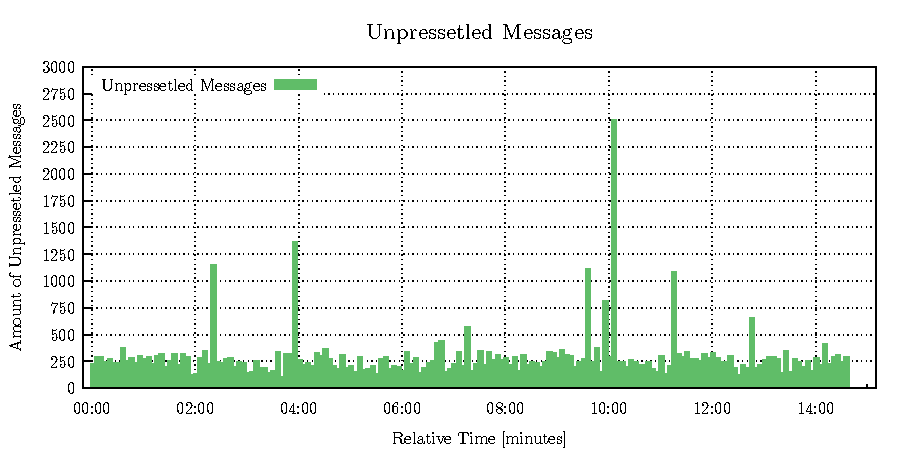
\includegraphics[width=\linewidth]{obrazky-figures/charts/singlepoint-router-throughput-routerLink.pdf}}
	\end{minipage}
	\begin{minipage}{0.49\linewidth}
		\subfloat[Topology with a single Broker node.\label{fig:router-multipoint-routerLink}]{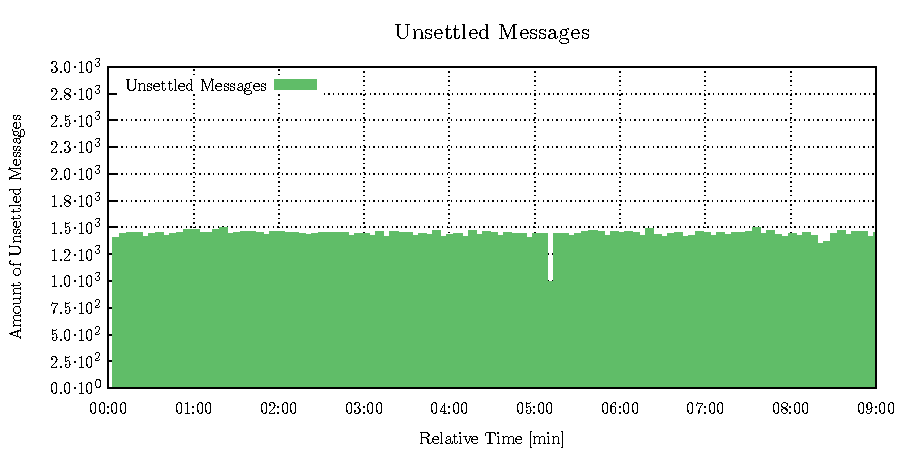
\includegraphics[width=\linewidth]{obrazky-figures/charts/multipoint-router-only-throughput-routerLink.pdf}}
	\end{minipage}
	\caption[Examples of experimental topologies created for basic performance testing and experiments with Maestro.]{Examples of experimental topologies created for basic performance testing and experiments with Maestro.}
  label{fig:routerLink-throughput}
\end{figure}

\section*{Latency}

Unpresettled messages for the router available in the Figure \ref{fig:latency-router-routerLink}. From the Inspector outputs one can see, that the Broker handled 10\,000\,000 messages in more than 7\,minutes, but the router handled the same amount of messages much faster approximately in 2\,minutes and 20\,seconds.

Since the router applies the flow control during this measurement and the rate is setup to 80\,\% of maximum, the unpressetled message count is here much lower than in the other cases as it is depicted in the Figure \ref{fig:latency-multiple-router-routerLink}.

\begin{figure}[h]
	\centering
	\begin{minipage}{0.49\linewidth}
		\subfloat[Single router node.\label{fig:latency-router-routerLink}]{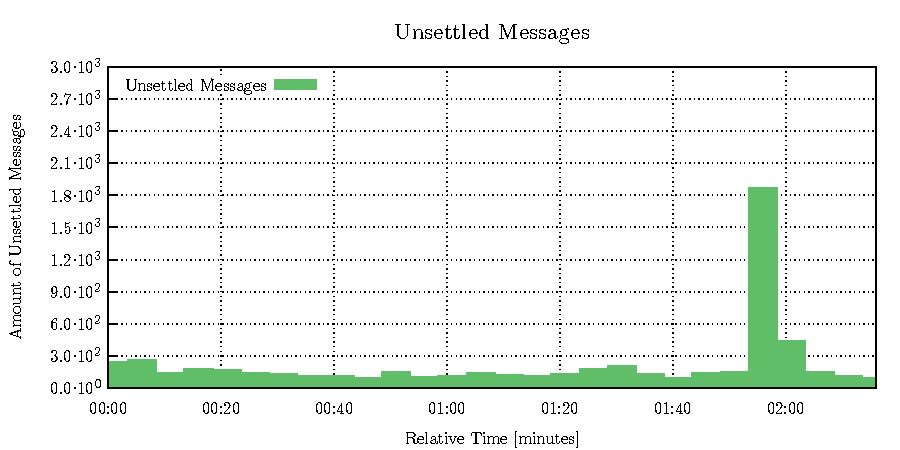
\includegraphics[width=\linewidth]{obrazky-figures/charts/singlepoint-router-latency-routerLink.pdf}}
	\end{minipage}
	\begin{minipage}{0.49\linewidth}
		\subfloat[Single Broker node.\label{fig:latency-multiple-router-routerLink}]{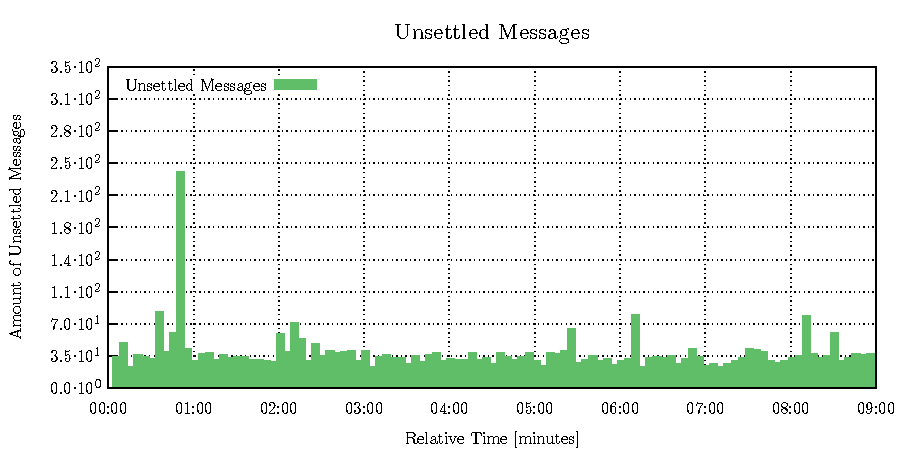
\includegraphics[width=\linewidth]{obrazky-figures/charts/multipoint-router-only-latency-routerLink.pdf}}
	\end{minipage}
	\caption[Examples of experimental topologies created for basic performance testing and experiments with Maestro.]{Examples of experimental topologies created for basic performance testing and experiments with Maestro.}\label{fig:routerLink-latency}
\end{figure}

\section*{Measurement With Redundant Router}

\begin{figure}[h]
	\centering
	\begin{minipage}{0.49\linewidth}
		\subfloat[Restart\label{fig:restart-redundant-agent-memory}]{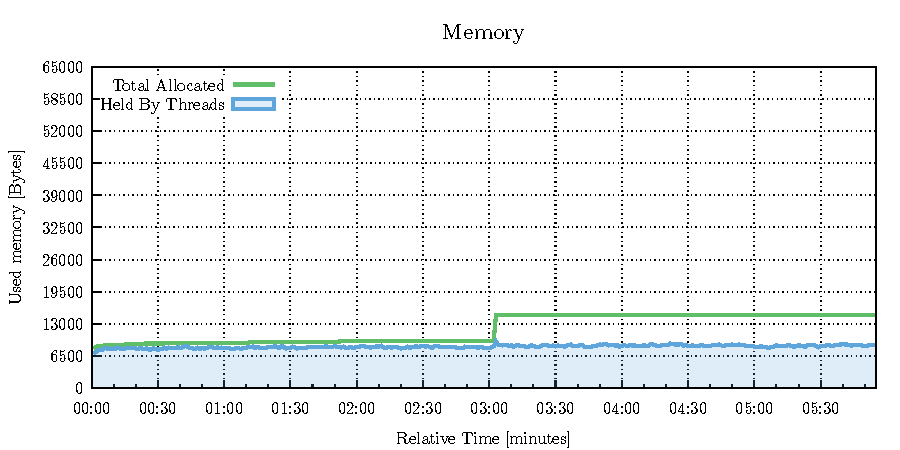
\includegraphics[width=\linewidth]{obrazky-figures/charts/restart-redundant-agent-memory.pdf}}
	\end{minipage}
	\begin{minipage}{0.49\linewidth}
		\subfloat[10 second shutdown\label{fig:shutdown_10-redundant-agent-memory}]{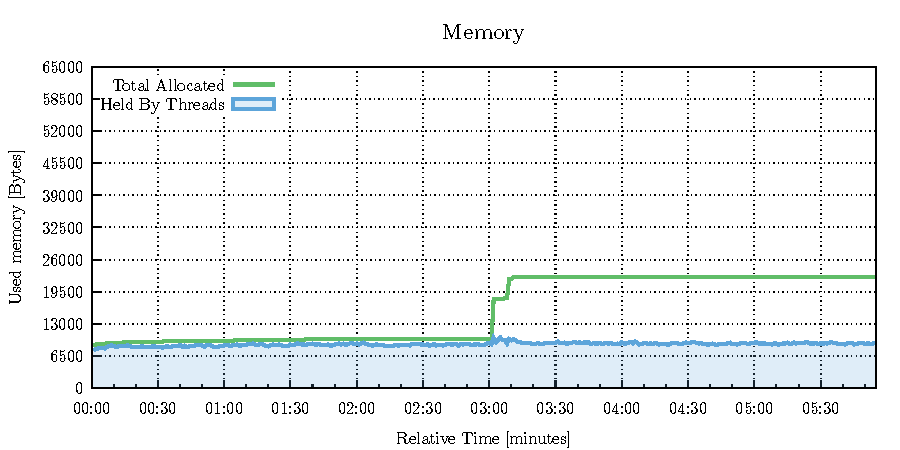
\includegraphics[width=\linewidth]{obrazky-figures/charts/shutdown_10-redundant-agent-memory.pdf}}
	\end{minipage}
  \begin{minipage}{0.49\linewidth}
		\subfloat[60 second shutdown\label{fig:shutdown_60-redundant-agent-memory}]{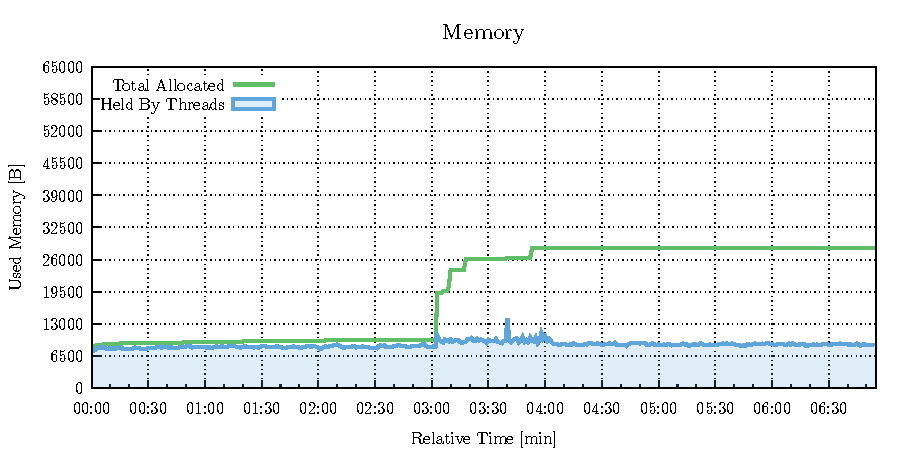
\includegraphics[width=\linewidth]{obrazky-figures/charts/shutdown_60-redundant-agent-memory.pdf}}
	\end{minipage}
	\begin{minipage}{0.49\linewidth}
		\subfloat[120 second shutdown\label{fig:shutdown_120-redundant-agent-memory}]{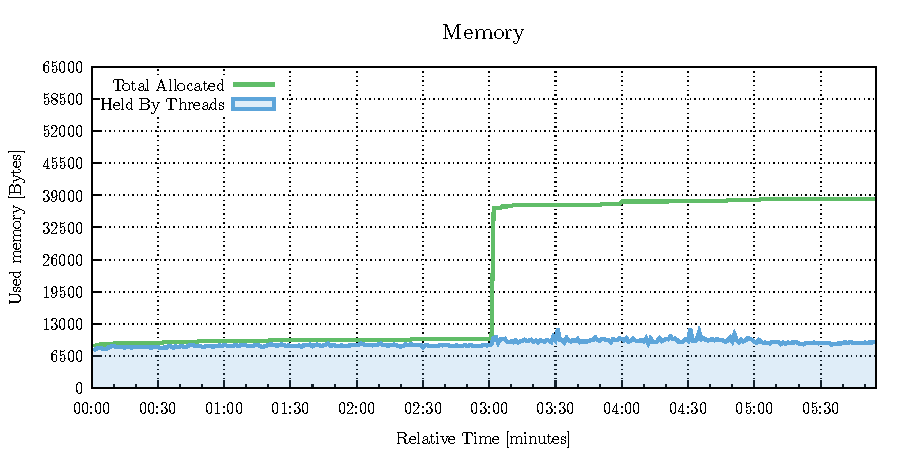
\includegraphics[width=\linewidth]{obrazky-figures/charts/shutdown_120-redundant-agent-memory.pdf}}
	\end{minipage}
	\caption[Collected data about the memory allocation for the redundant router node during the Agent actions execution.]{Collected data about the memory allocation for the redundant router node during the Agent actions execution.}\label{fig:redundant-memory-info}
\end{figure}

\begin{figure}[h]
	\centering
	\begin{minipage}{0.49\linewidth}
		\subfloat[Restart\label{fig:restart-redundant-agent-routerLink}]{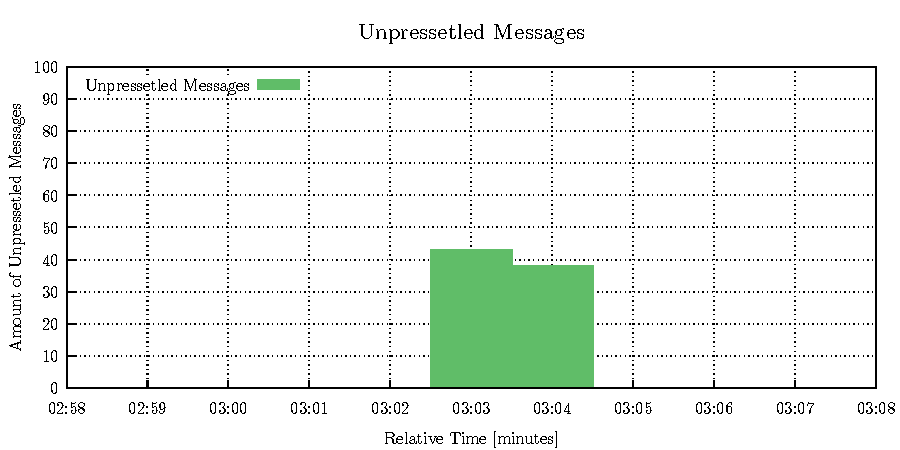
\includegraphics[width=\linewidth]{obrazky-figures/charts/restart-redundant-agent-routerLink.pdf}}
	\end{minipage}
	\begin{minipage}{0.49\linewidth}
		\subfloat[10 second shutdown\label{fig:shutdown_10-redundant-agent-routerLink}]{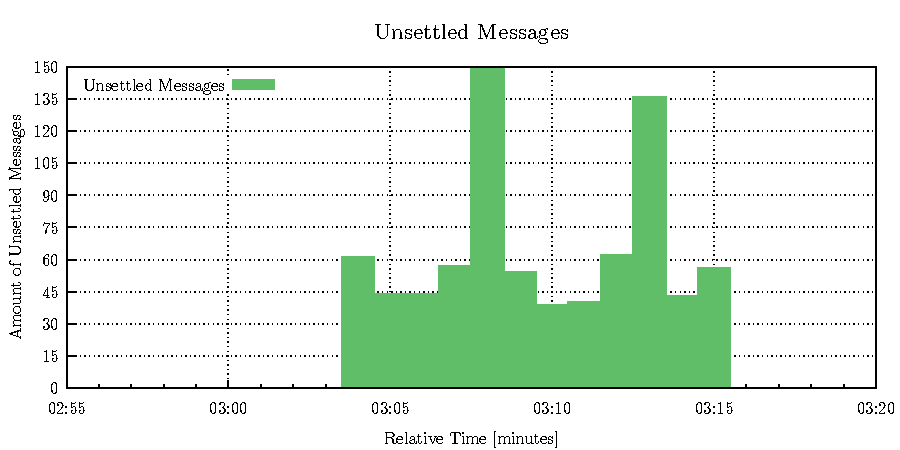
\includegraphics[width=\linewidth]{obrazky-figures/charts/shutdown_10-redundant-agent-routerLink.pdf}}
	\end{minipage}
  \begin{minipage}{0.49\linewidth}
		\subfloat[60 second shutdown\label{fig:shutdown_60-redundant-agent-routerLink}]{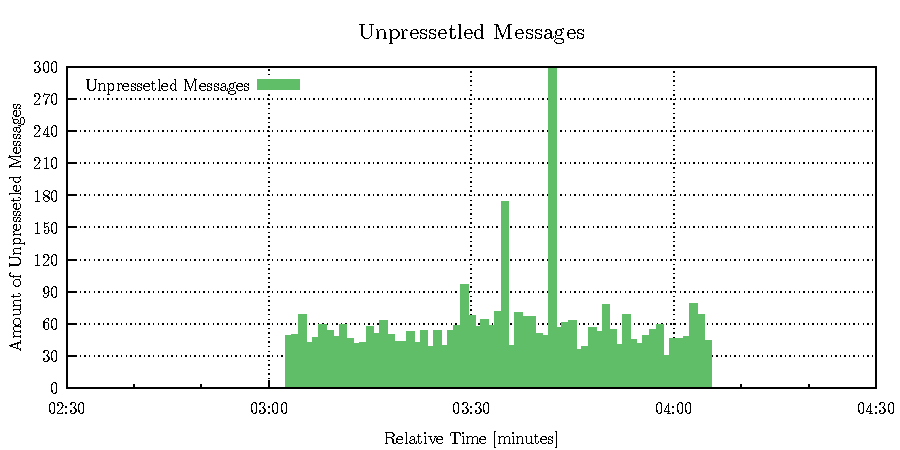
\includegraphics[width=\linewidth]{obrazky-figures/charts/shutdown_60-redundant-agent-routerLink.pdf}}
	\end{minipage}
	\begin{minipage}{0.49\linewidth}
		\subfloat[120 second shutdown\label{fig:shutdown_120-redundant-agent-routerLink}]{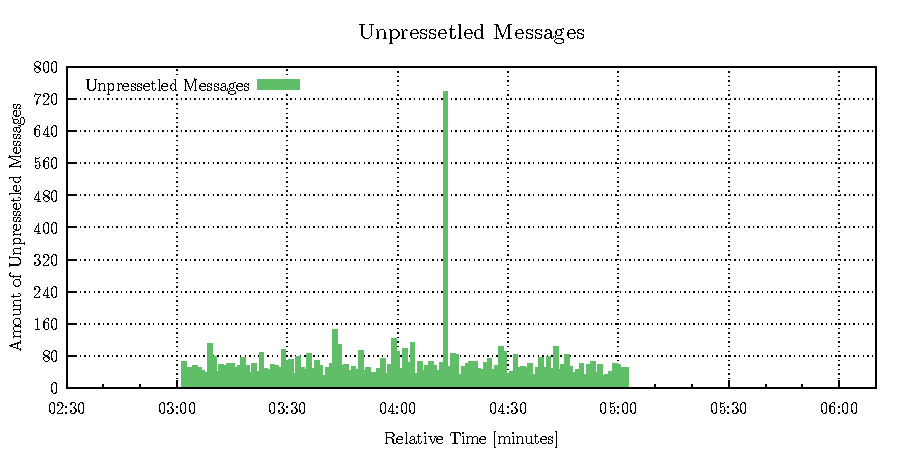
\includegraphics[width=\linewidth]{obrazky-figures/charts/shutdown_120-redundant-agent-routerLink.pdf}}
	\end{minipage}
	\caption[Collected data about the unpressetled messages for the redundant router node during the Agent actions execution.]{Collected data about the unpressetled messages for the redundant router node during the Agent actions execution.}\label{fig:routerLink-latency}
\end{figure}

\begin{figure}[h]
	\centering
	\begin{minipage}{0.49\linewidth}
		\subfloat[Restart\label{fig:restart-redundant-agent-delivered}]{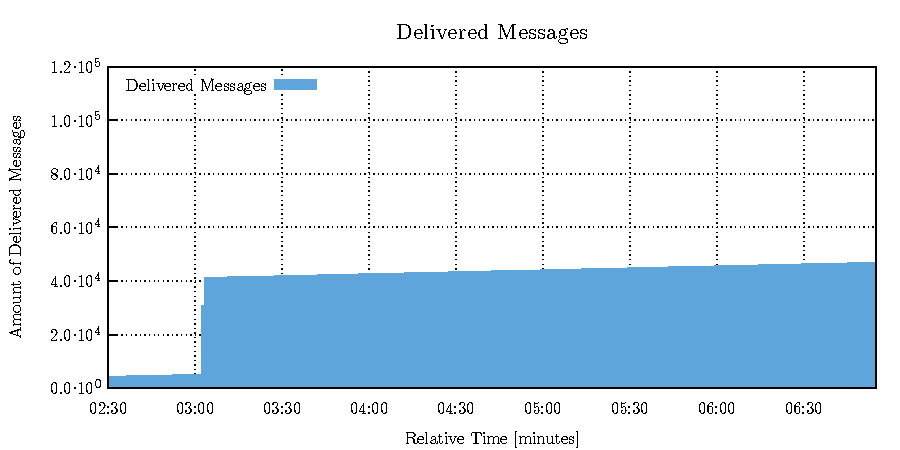
\includegraphics[width=\linewidth]{obrazky-figures/charts/restart-redundant-agent-delivered.pdf}}
	\end{minipage}
	\begin{minipage}{0.49\linewidth}
		\subfloat[10 second shutdown\label{fig:shutdown_10-redundant-agent-delivered}]{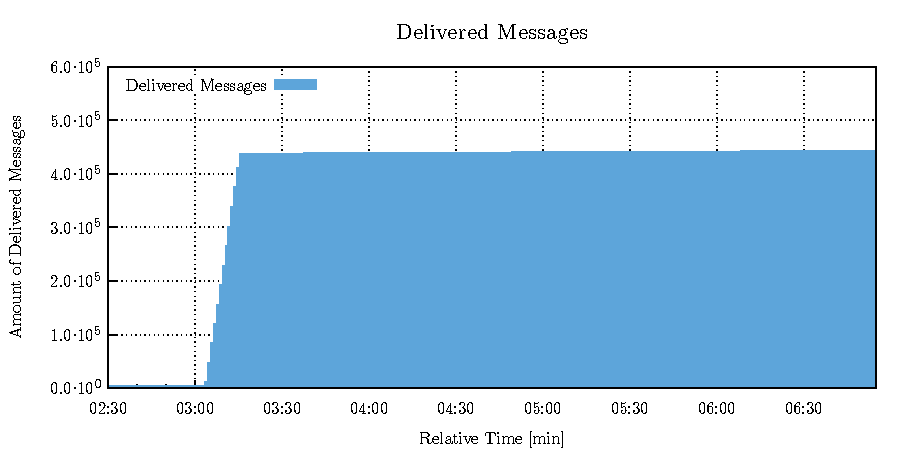
\includegraphics[width=\linewidth]{obrazky-figures/charts/shutdown_10-redundant-agent-delivered.pdf}}
	\end{minipage}
  \begin{minipage}{0.49\linewidth}
		\subfloat[60 second shutdown\label{fig:shutdown_60-redundant-agent-delivered}]{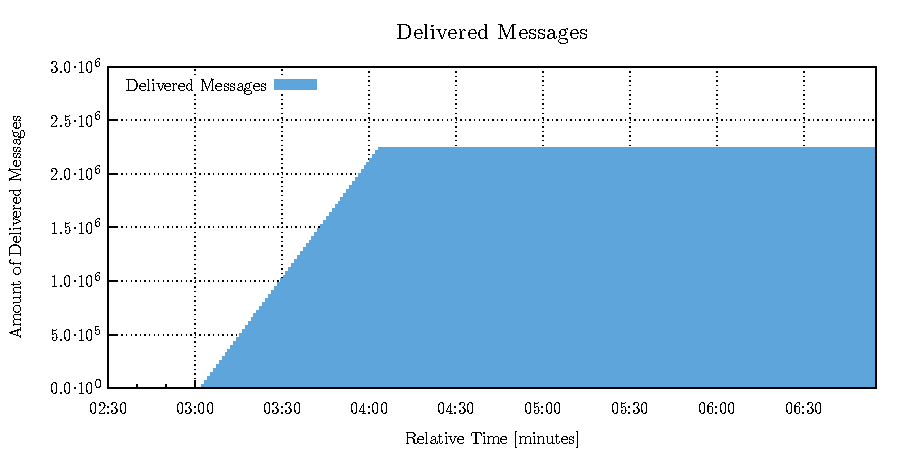
\includegraphics[width=\linewidth]{obrazky-figures/charts/shutdown_60-redundant-agent-delivered.pdf}}
	\end{minipage}
	\begin{minipage}{0.49\linewidth}
		\subfloat[120 second shutdown\label{fig:shutdown_120-redundant-agent-delivered}]{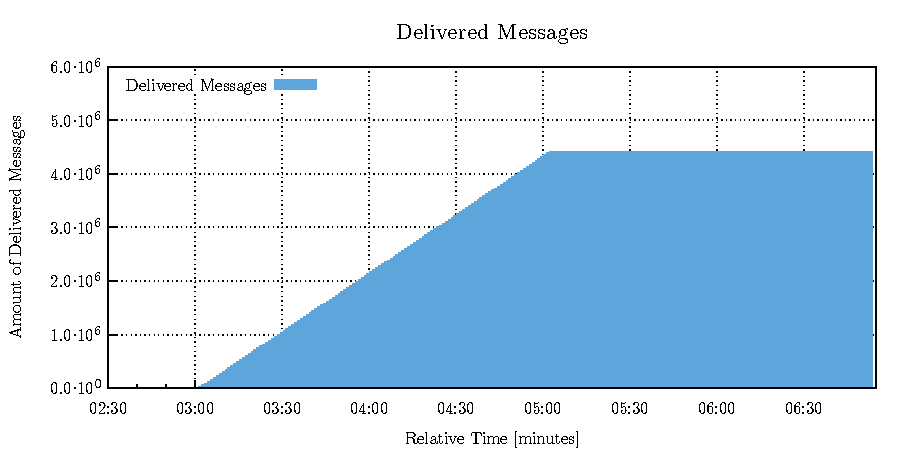
\includegraphics[width=\linewidth]{obrazky-figures/charts/shutdown_120-redundant-agent-delivered.pdf}}
	\end{minipage}
	\caption[Collected data about the delivered messages for the redundant router node during the Agent actions execution.]{Collected data about the delivered messages for the redundant router node during the Agent actions execution.}\label{fig:routerLink-latency}
\end{figure}



%\chapter{RelaxNG Schéma konfiguračního souboru} % Scheme of RelaxNG configuration file

%\chapter{Plakát} % poster
